\chapter*{Introduction au cours LINGI1101}

Le cours "\textit{Logique et Structures discrètes"} a deux buts importants:

\begin{itemize}
\item Donner la motivation et l'intuition de la logique, pour que cette matière devienne véritablement utile pour les étudiants.
\item Donner les concepts et les formalismes mathématiques nécessaires pour utiliser la logique à bon escient.
\end{itemize}


L'intuition est donc importante pour ce cours, néanmoins, la connaissance des formalismes mathématiques reste essentielle.  Le cours sera coté sur les deux: intuitions (un tiers) et formalismes (deux tiers).\\

\section*{Déroulement du cours}

Le cours est composé de deux parties. La première partie, \textit{logique formelle}, représentera deux tiers du cours. La seconde partie, \textit{structures discrètes sur Internet}, comptera quant à elle pour un tiers du cours.\\

L'évaluation de ce cours se compose de trois parties. Il y aura tout d'abord une interrogation au milieu du quadrimestre portant sur 5 points. Il vous sera également demandé de prendre note pendant une heure de cours par groupe de trois, ceci afin de contribuer au syllabus. Ces notes prises au cours rapporteront au maximum 2 points de la note finale à chacun des participants. L'examen sera divisé en deux parties. La première partie sur 5 points portera sur la matière de l'interrogation. La note retenue sera le maximum entre la note de l'interrogation et celle obtenue à la question de l'examen. La seconde partie de l'examen sera donc cotée sur 13 points et portera sur le reste de la matière.\\

Afin de suivre ce cours, nous nous baserons sur deux livres de référence correspondants chacun à une partie du cours :

\begin{itemize}
\item Introductory Logic and Sets for Computer Scientists, by \textit{Nimal Nissanke}.
\item Networks, Crowds, and Markets: Reasoning About a Highly Connected World, by \textit{David Easley and Jon Kleinberg}. \footnote{Quelques chapitres.}
\end{itemize}

La première partie sera complétée par des sujets et exercices plus avancés qui approfondissent le traitement du livre.

\section*{Plan du cours}

Cette partie va parler du rôle des raisonnements et des différentes formes de raisonnement. Nous prendrons en exemple la méthode scientifique.

\subsection*{Logique des propositions}

La logique des propositions est un langage formel constitué d'une syntaxe et d'une sémantique. La syntaxe décrit l'ensemble des formules qui appartiennent au langage. La sémantique permet de donner un sens aux formules de langage. C'est une logique très ancienne qui vient de l'antiquité. 

\subsection*{Logique des prédicats}

C'est la logique la plus expressive et la plupart des travaux mathématiques peuvent être écrits dans ce langage. Elle est aussi définie comme la logique du premier ordre.\footnote{Il existe d'autres formes de logiques plus expressives, mais plus difficiles à utiliser. Exemple : la logique du deuxième ordre. } En logique des prédicats, les éléments de base du langage ne sont plus des propositions, mais des prédicats. 

\subsection*{Interprétations et modèles}

La logique a besoin d'un langage, de phrases pour la décrire. Cette section couvrira donc la sémantique à utiliser.

\subsection*{Théorie de preuve}

Nous pouvons manipuler une phrase en logique pour obtenir un résultat. Par exemple, si A et B sont vrais, nous pouvons en déduire que A est vrai. Il y a des règles d'inférences à utiliser pour prendre une phrase en logique et en déduire une autre.
Une preuve mathématique est une séquence de phrases liées par des règles d'inférences.

\subsection*{Algorithme de preuve}
C'est l'algorithme le plus puissant qui existe en logique des prédicats. Néanmoins, il est inefficace seul. Afin de le rendre efficace, il faut poser des hypothèses. Nous approfondirons ce problème dans le cadre de cette section. 

\subsection*{Théorie logique}

Il est possible de formaliser tout objet mathématique avec une théorie logique qui lui est propre.  En exemple, citons la théorie des ensembles, des fonctions et des ordres partiels.

\subsection*{Programmation logique}

Le rêve serait de pouvoir exprimer toute chose logique en langage de programmation efficace. Il s'agira d'appliquer ce principe avec l'algorithme de preuve, sur base d'hypothèses.

\part{Logique formelle}
\chapter{Contexte: la méthode scientifique}

\section{Formalisation d'un système}

Comment pouvons-nous formaliser un système dans le monde réel tels que les champs magnétiques ou la gravitation ?

\begin{center}
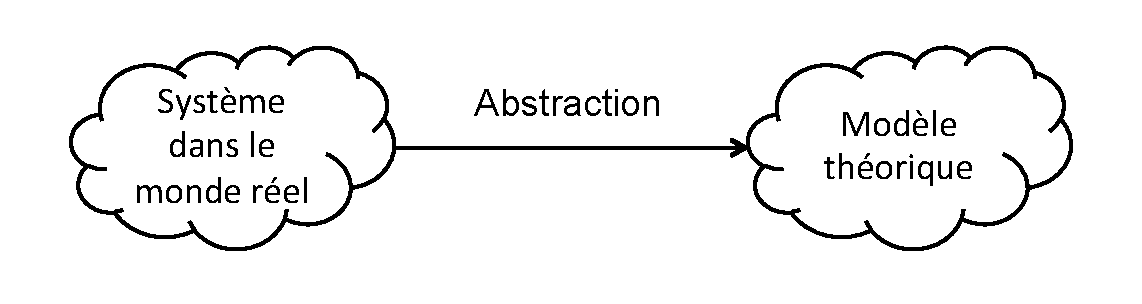
\includegraphics[scale=0.65]{images/Abstraction.pdf}
\end{center}

Afin de formaliser un système dans le monde réel, nous devons faire une abstraction vers un modèle théorique. Ce modèle théorique est un ensemble de phrases logiques dont il est possible de tirer des prédictions. Il n'est intéressant que s'il se comporte comme le vrai système.

Un exemple de cette formalisation pourrait être les équations de Maxwell qui sont le modèle théorique correspondant à la trajectoire des électrons et protons.

\section{Boucle de raisonnement}

Il existe trois formes de raisonnement: la déduction, l'induction et l'abduction. Ces trois formes de raisonnement peuvent être liées dans une boucle de raisonnement de la façon suivante:

\begin{center}
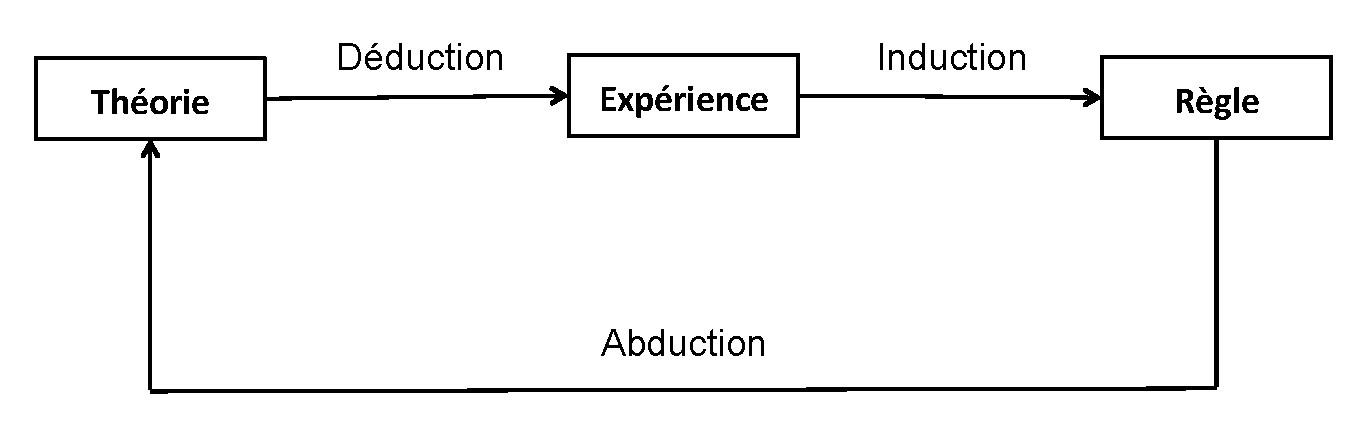
\includegraphics[scale=0.50]{images/BoucleRaisonnement1.pdf}
\end{center}

\subsection{Déduction}

Il s'agit de faire des calculs et des raisonnements logiques par rapport à la théorie. On en conclut une expérience. \\

\subsection{Induction}

L'induction est le fait de trouver une règle générale qui décrit les résultats d'expériences. On choisit en général une règle moyenne qui deviendra la règle générale.  Il faut souligner que les résultats expérimentaux ne sont pas totalement fiables ou incomplets. Dès lors, la règle trouvée n'est pas nécessairement exacte.  Par exemple, si par induction nous avons trouvé la règle, "les oiseaux volent", cela est vrai tant que l'on n’a pas vu un pingouin. Autre exemple, nous pouvons supposer que demain le soleil va se lever comme depuis des milliers d'années, même si rien ne l'assure.\\

\subsection{Abduction}

On compare la règle générale trouvée lors de l'induction avec la théorie. Si cela se révèle différent, comme l'on suppose que tout est parfait dans les calculs/expériences, c'est la théorie qui est fausse. Il faut alors corriger la théorie existante ou en inventer/deviner une nouvelle. Ce type de raisonnement est l'abduction. On applique l'abduction couramment dans notre vie de tous les jours; par exemple, lorsqu'un élève entre trempé dans la classe, nous supposons qu'il pleut dehors. \\


Sur ces trois concepts, seule la déduction est un raisonnement sûr, les deux autres sont encore mal compris. Nous nous focaliserons dans ce cours uniquement sur la déduction. \\


\section{Exemples}

\subsection{Loi de Maxwell}

Nous illustrons dès à présent le fonctionnement de la boucle de raisonnement à l'aide de l'exemple cité plus haut, c'est-à-dire les équations de Maxwell :

\begin{center}
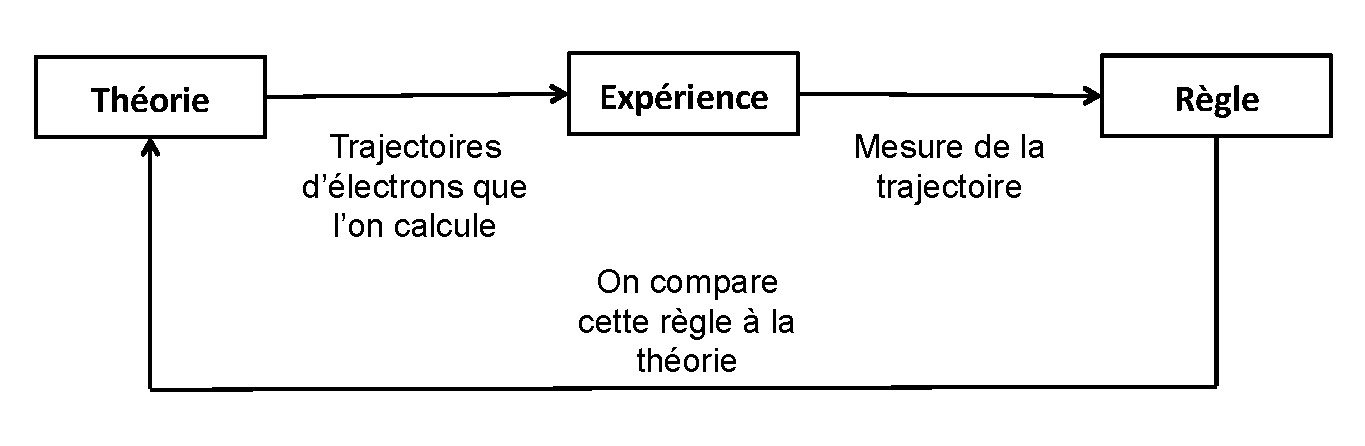
\includegraphics[scale=0.50]{images/BoucleRaisonnement2.pdf}
\end{center}

Par déduction, grâce à la théorie et aux conditions initiales que nous fixons, nous trouvons la trajectoire d'un électron. Nous effectuons ensuite des mesures dans le monde réel. Nous allons, par exemple, mesurer la trajectoire plusieurs fois avec des méthodes différentes et, par induction, nous trouvons une règle qui est la loi de comportement de la particule. Nous comparons ensuite, par abduction, cette règle à la théorie, et nous la corrigeons si besoin.\\



\subsection{Sac de billes}

Afin d'illustrer les 3 formes de raisonnements de manière plus formelle, considérons un sac de billes pouvant contenir des billes noires ou blanches. Notons que sac(x) signifie "la bille x est dans le sac" et que blanc(x) signifie "la bille x est blanche". \\

\subsubsection{Déduction}

\begin{enumerate}
  \item Règle: $\forall$ $x$, $sac(x)$ $\Rightarrow$ $blanc(x)$
  \item Cas: $sac(a)$, $sac(b)$, $\cdots$\\
  \rule{5.5cm}{.1pt} 
  \item Résultat: $blanc(a)$, $blanc(b)$, $\cdots$
\end{enumerate}

Si toutes les billes se trouvant dans le sac sont blanches et que l'on pioche une bille de ce sac, cette bille sera blanche. Cette déduction est forcément correcte.

\subsubsection{Induction}

\begin{enumerate}
  \item Cas: $sac(a)$, $sac(b)$,$\cdots$
  \item Résultat: $blanc(a)$, $blanc(b)$, $\cdots$\\
  \rule{5.5cm}{.1pt}	
  \item Règle: $\forall$ $x$, $sac(x)$ $\Rightarrow$ $blanc(x)$
\end{enumerate}

Si toutes les billes qu'on l'on pioche du sac sont blanches, alors nous pouvons établir comme règle que toutes les billes dans le sac sont blanches. Cette induction n'est pas forcément correcte.

\subsubsection{Abduction}

\begin{enumerate}
  \item Règle: $\forall$ $x$, $sac(x)$ $\Rightarrow$ $blanc(x)$
  \item Résultat: $blanc(a)$, $blanc(b)$, $\cdots$\\
  \rule{5.5cm}{.1pt}
  \item Cas: $sac(a)$, $sac(b)$, $\cdots$
\end{enumerate}

Si toutes les billes se trouvant dans le sac sont blanches et que nous trouvons des billes blanches à côté du sac, nous pouvons penser qu'elles viennent du sac. Cette abduction n'est pas forcément correcte.
